\documentclass[german]{tum-presentation}

\usepackage[utf8]{inputenc}
\usepackage[ngerman]{babel}
\usepackage[autostyle]{csquotes}
\usepackage[T1]{fontenc}
\usepackage{amsmath}
\usepackage{amsfonts}
\usepackage{amssymb}
\usepackage{float}
\usepackage{graphicx}
\usepackage{booktabs}
\usepackage{icomma}
\usepackage{siunitx}
\usepackage{multicol}
\usepackage[german]{varioref}
\usepackage{listings}
\usepackage{color}

% setup commands
\newcommand*\diff{\mathop{}\!\mathrm{d}}
\newcommand*\Diff[1]{\mathop{}\!\mathrm{d^#1}}
\newcommand{\define}[2]{\item \textbf{#1}\\#2}
\newcommand{\conclude}[0]{\ensuremath{\Longrightarrow} }
\newcommand{\refer}[0]{\ensuremath{\rightarrow} }
\sisetup{range-phrase=--,range-units=single}
\MakeOuterQuote{"}

% config for source code listings
\lstset{
	language=C++,
	aboveskip=3mm,
	belowskip=3mm,
	showstringspaces=false,
	columns=flexible,
	basicstyle={\ttfamily},
	breaklines=true,
	breakatwhitespace=true,
	tabsize=3
}

% bibliography
\addbibresource{literature.bib}

% document properties
\title[Binary Translation: RISC--V \refer x86--64]{Dynamische Binärübersetzung: RISC--V \refer x86--64}
\subtitle{Zwischenpräsentation}
\author[Dormann, Kammermeier, Pfannschmidt, Schmidt]{Noah Dormann\inst{1}, Simon Kammermeier\inst{1},\\Johannes Pfannschmidt\inst{1}, Florian Schmidt\inst{1}}
\institute[]{\inst{1} Fakultät für Informatik,
  Technische Universität München (TUM)}
\date{21. Juli 2020}

% beamer setup
\footline{\insertshortauthor~|~\insertshorttitle}
\setbeamertemplate{section in toc}[sections numbered]
\setbeamertemplate{subsection in toc}[subsections numbered]

\begin{document}

\begin{frame}[noframenumbering]
 	\titlepage
\end{frame}

\begin{frame}
	\frametitle{Gliederung}
	\tableofcontents
\end{frame}

% selbstverständlich sample-Gliederung
\section{Einführung} % Noah
\subsection{Dynamische Binärübersetzung}
\begin{frame}
	\frametitle{Einführung}
	\framesubtitle{Dynamische Binärübersetzung}
	Was ist dynamische Binärübersetzung?
	\begin{itemize}
			\item lazy - Befehle werden erst übersetzt, wenn sie tatsächlich ausgeführt werden sollen
			\item manche Teile des Codes werden möglicherweise gar nicht übersetzt
	\end{itemize}	
\end{frame}
\subsection{Grobüberblick über die RISC--V ISA}
\begin{frame}
	\frametitle{Einführung}
	\framesubtitle{Grobüberblick über die RISC--V ISA}
	\begin{itemize}
		\item x86-64: CISC \refer complex instruction set
		\begin{itemize}
			\item Register-Memory-Architektur 
			\item 16 GPRs
			\item 2-Adressform
		\end{itemize}
		\item RISC-V: RISC \refer reduced instruction set
		\begin{itemize}
			\item Load-Store-Architektur 
			\item 31 GPRs
			\item 3-Adressform
			\item spezielles Zero-Register
		\end{itemize}
	\end{itemize}

\end{frame}
\subsection{Angebot}

\section{Systemarchitektur}
\begin{frame}
	\frametitle{Systemarchitektur}
	\begin{figure}
		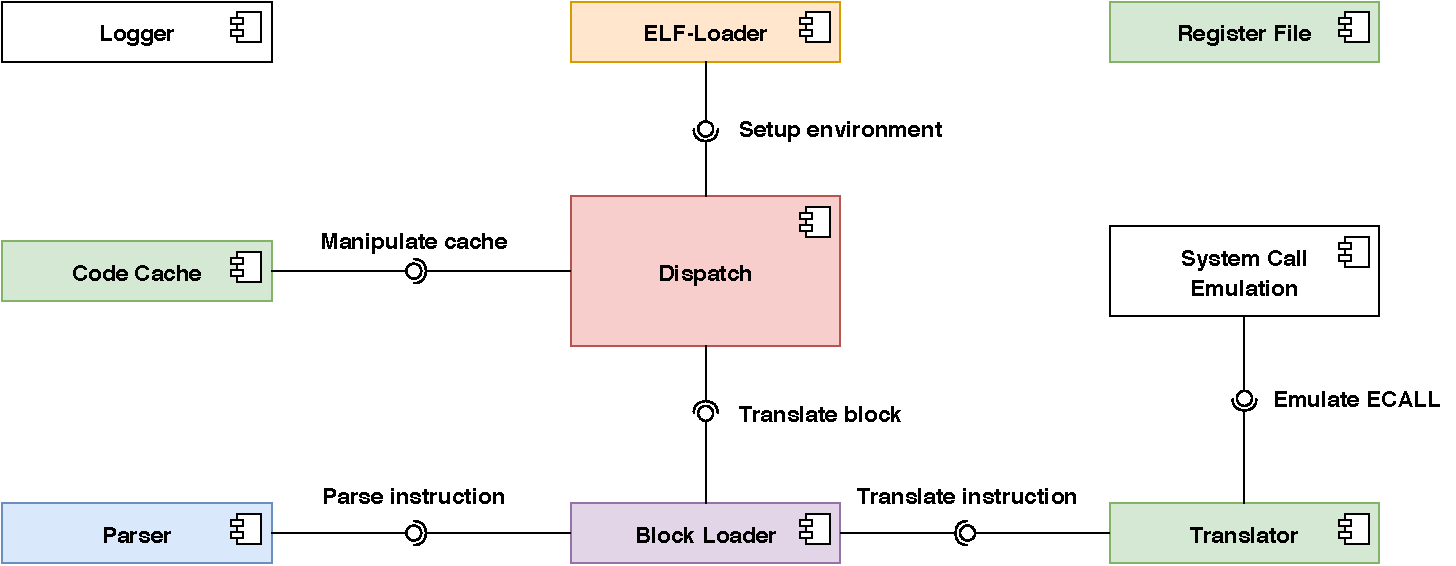
\includegraphics[width=0.96\textwidth]{diagrams/components}
	\end{figure}
\end{frame}

\begin{frame}
	\frametitle{Programmablauf}
	\begin{figure}
		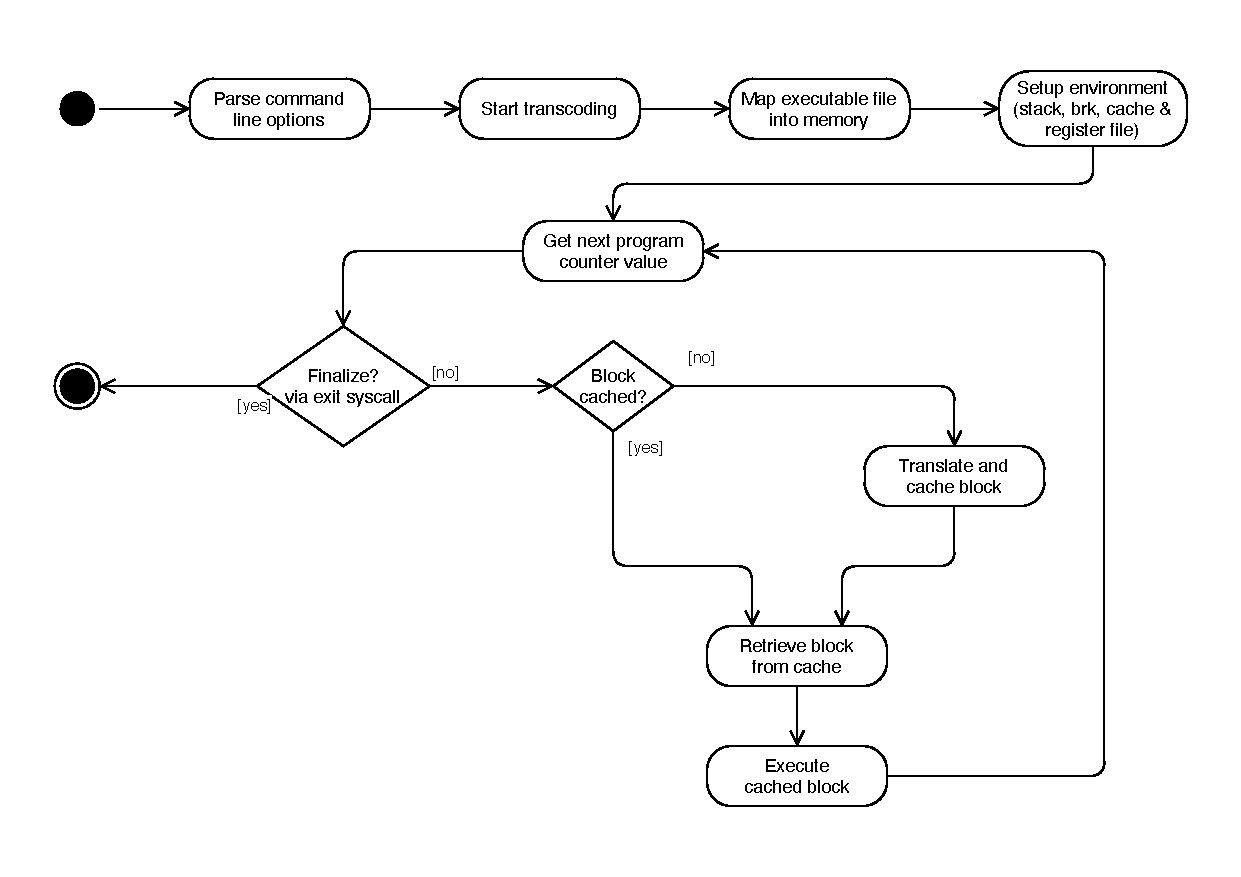
\includegraphics[width=\textwidth]{diagrams/strategy}
	\end{figure}
\end{frame}

\subsection{ELF-Loader} % Simon
\begin{frame}
	\frametitle{ELF-Loader}
	\framesubtitle{Überblick}
	\textbf{Aufgabe:} Speicher für das Gastprogramm anlegen und mit Startwerten, Instruktionen, etc. befüllen

	\vspace{0.25cm}
	Aufgeteilt in:
	\begin{itemize}
		\item Memory mapping
		\item Stack Allocation
	\end{itemize}
\end{frame}


\begin{frame}[fragile]
	\frametitle{ELF-Loader}
	\framesubtitle{Memory mapping}
	\textbf{Ziel:} Die Binärdatei einlesen und alle Segmente, die mit "load" gekennzeichnet sind, an die korrekten Orte im Speicher laden.

	\vspace{0.25cm}
	\textbf{Input:} String des Pfads der Binärdatei.

	\textbf{Output:} Einsprungadresse des geladenen RISCV-Programms (plus einige Metadaten) in einem \verb!t_risc_elf_map_result! struct.

	\vspace{0.25cm}

	\begin{columns}[onlytextwidth]

		\onslide<2->
		\begin{column}{0.49\textwidth}
			\begin{itemize}
				\item Laden des ELF-Headers vom Anfang der Datei.
				\item Checken der Flags auf nicht unterstüzte RISCV ABIs
				\item Iterieren über alle Segment-Header um den Addressbereich des Binarys zu erhalten
				\item Allozieren des gesamten benötigten Addressbereichs an der nativen Addresse
				\item Laden aller "load" Segmente an die richtigen Speicheradressen
			\end{itemize}
		\end{column}
		\onslide<1->
		\begin{column}{0.49\textwidth}
			\begin{lstlisting}
				typedef struct {
   					bool valid;
    					t_risc_addr entry;
    					t_risc_addr phdr;
    					Elf64_Half ph_count;
    					Elf64_Half ph_entsize;
    					t_risc_addr dataEnd;
				} t_risc_elf_map_result;
			\end{lstlisting}
		\end{column}
	\end{columns}
\end{frame}

\begin{frame}[fragile]
	\frametitle{ELF-Loader}
	\framesubtitle{Stack Allocation}
	\textbf{Ziel:} Stack für das Gastprogramm allozieren und mit den üblichen Daten initialisieren.

	\vspace{0.25cm}
	\textbf{Input:} Argumentanzahl des Gastprogramms, Argumentarray des Gastprogramms, der Output des memory mappings

	\textbf{Output:} Die Adresse des Stackpointers nach dem Initialisieren

	\pause
	%\vspace{0.5cm}
	\begin{columns}[c, onlytextwidth]
		\begin{column}{0.49\textwidth}
			\begin{itemize}
				\only<2>{\item Allozieren von Speicher für das Stack entsprechend des stack limits des Kernels (oder 8 MiB als Standardwert)}
				\item<3-> Guard page am unteren Ende des Stacks um Overflow abzufangen.
				\item<3-> Alignment, damit der resultierende Stack Pointer die ABI erfüllt (16 Byte aligned)
				\item<3-> Kopieren der Werte des auxiliary vectors (aus Resultat des memory mappings bzw. Daten des Hostprogramms)
				\item<3-> Kopieren des enviroment vectors des Hostprogramms
				\item<3-> Kopieren des Argumentarrays und der Argumentanzahl
			\end{itemize}
		\end{column}

		\begin{column}{0.49\textwidth}

			\centering
			\onslide<3->
			\begin{tabular}{|c|}
				\hline
				\rule[-1ex]{0pt}{3ex} \vdots                                      \\
				(Nicht Teil des Stacks)                                               \\
				\hline
				\rule[-1ex]{0pt}{3ex} Stack Alignment                                 \\
				\hline
				\rule[-1ex]{0pt}{3ex} Null terminierter auxiliary vector              \\
				\hline
				\rule[-1ex]{0pt}{3ex} Null terminierter enviroment vector             \\
				\hline
				\rule[-1ex]{0pt}{3ex} Null terminierter Argumentarray                 \\
				\hline
				\rule[-1ex]{0pt}{3ex} Argumentanzahl (Stack Pointer am Ende auf hier) \\
				\hline
				\rule[-1ex]{0pt}{3ex} \vdots                                          \\
				\hline
				\rule[-1ex]{0pt}{3ex} Guard page                                      \\
				\hline
			\end{tabular}
		\end{column}
	\end{columns}
\end{frame}

\subsection{Parser} % Noah
\begin{frame}[fragile]
	\frametitle{Parser}
	\framesubtitle{Überblick}
	\textbf{Ziel:} Dekodieren der 4 Byte großen kodierten RISC-V-Befehle aus der geladenen ELF-Datei.

	\refer (Zählen der Anzahl von Zugriffen auf einzelne Register für spätere Optimierungen.)

	\vspace{0.25cm}
	\textbf{Input:} Zeiger auf RISC-V-Befehl im Speicher

	\textbf{Output:} Ausgefüllte \verb!t_risc_instr! Struktur mit allen relevanten Informationen
	
	\pause

	\begin{columns}
		\begin{column}{0.4\textwidth}
			\begin{lstlisting}
				typedef struct {
				    t_risc_addr addr;
				    t_risc_mnem mnem;
				    t_risc_optype optype;
				    t_risc_reg reg_src_1;
				    t_risc_reg reg_src_2;
				    t_risc_reg reg_dest;
				    t_risc_imm imm;
				} t_risc_instr;
			\end{lstlisting}
		\end{column}
		\begin{column}{0.6\textwidth}
			\vspace{0.25cm}
			\begin{itemize}
				\item \verb!addr! \refer Addresse des originalen riscv-Befehls im Speicher				
				\item \verb!mnem! \refer Mnemonic der Instruktion (Zusammengesetzt aus Opcode und weiteren \textit{funct} Blöcken)
				\item \verb!optype! \refer Optype (Kategorie der Instruktion)
				\item \verb!reg_(dest/src1/src2)! \refer Registernummern der Quell- und Ziel Register
				\item \verb!imm! \refer Immediate der Instruktion
			\end{itemize}
		\end{column}
	\end{columns}


\end{frame}

\begin{frame}[fragile]
	\frametitle{Parser}
	\framesubtitle{Extrahieren der Blöcke}
	\textbf{Ziel:} Dekodieren der 4 Byte großen kodierten RISC-V-Befehle aus der geladenen ELF-Datei.
	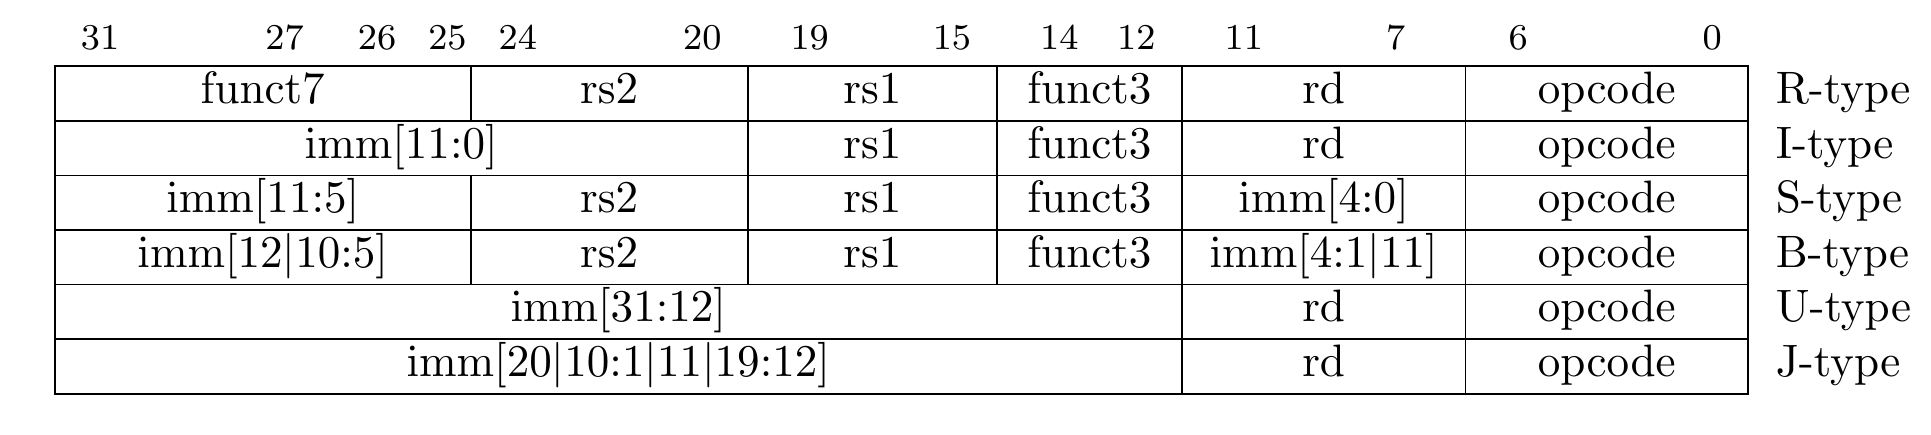
\includegraphics[width=0.99\textwidth]{diagrams/optypes}
	\footfullcite{riscv-spec}
	\pause
	Um die einzelnen Teile der Instruktion zu extrahieren verwenden wir kompakte inline Funktionen. 
	\begin{lstlisting}
	// extract U-Type immediate bit[31:12] -> mask lower 12 bit [11:0] with zeros
	static inline int extract_imm_U(int32_t instr) { return instr & ~(0xfff); }
	\end{lstlisting}
\end{frame}

\begin{frame}[fragile]
	\frametitle{Parser}
	\framesubtitle{Umsetzung}
	\textbf{Ziel:} Dekodieren der 4 Byte großen kodierten RISC-V-Befehle aus der geladenen ELF-Datei.
	\begin{lstlisting}
	void parse_instruction(t_risc_instr *p_instr_struct, uint32_t *reg_count);
	\end{lstlisting}
	Zunächst wird der Opcode extrahiert, dieser legt das Format (R/I/S/B/U/J-type) fest.
	
	Teilweise lässt sich die Mnemonic schon exakt aus dem Opcode auslesen (U/J-type).
	\begin{lstlisting}
    int32_t raw_instr = *(int32_t *) p_instr_struct->addr; //cast and dereference
    p_instr_struct->reg_dest = extract_rd(raw_instr);      //fill basic struct
    t_opcodes opcode = raw_instr >> 2 & 0x1f;				//extract opcode bits[6:2]
    switch (opcode) {
        case OP_LUI:
            p_instr_struct->optype = UPPER_IMMEDIATE;
            p_instr_struct->mnem = LUI;
            p_instr_struct->imm = extract_imm_U(raw_instr);
            break;
        //...
    }
	\end{lstlisting}
\end{frame}

\begin{frame}[fragile]
	\frametitle{Parser}
	\framesubtitle{Umsetzung}
	\textbf{Ziel:} Dekodieren der 4 Byte großen kodierten RISC-V-Befehle aus der geladenen ELF-Datei.
	\begin{lstlisting}
	void parse_instruction(t_risc_instr *p_instr_struct, uint32_t *reg_count);
	\end{lstlisting}
	Bei einigen Instruktionen muss zusätzlich zwischen den \textit{funct} Codes unterschieden werden.
	\begin{lstlisting}
    case OP_OP_IMM_32:
            p_instr_struct->optype = IMMEDIATE;
            switch (extract_funct3(raw_instr)) {
                case 0:
                    p_instr_struct->mnem = ADDIW;
                    p_instr_struct->imm = extract_imm_I(raw_instr);
                    break;
                //...
            }
            break;
	\end{lstlisting}
\end{frame}



\subsection{Register File} % Flo
\begin{frame}[fragile]
	\frametitle{Register File}
	\textbf{Ziel:} Speicherung der Registerinhalte des RISC-V-Programmes
	
	\vspace{1cm}
	\pause
	Emulieren der Register \verb!x0! bis \verb!x31! sowie \verb!pc! in
	\begin{lstlisting}
		t_risc_reg_val contents[33];
	\end{lstlisting}
	
	\pause
	und Zugriff via Startpointer und den Zugriffsmethoden:
	
	\begin{lstlisting}
		t_risc_reg_val *get_reg_data(void);
		t_risc_reg_val get_value(t_risc_reg reg);
		void set_value(t_risc_reg reg, t_risc_reg_val val);
	\end{lstlisting}
	
	z.T.: Caching der Inhalte in Hardware-x86-Registern je nach Registermapping für die Basic Blocks.
\end{frame}

\subsection{Block Loader} % Johannes
\begin{frame}[fragile]
\frametitle{Block Translator}
\framesubtitle{Vorgehen}
\begin{columns}[T]
	\begin{column}{0.7\textwidth}
		\textbf{Aufgabe:}    Basic Blocks parsen, übersetzen, und im Cache ablegen
		\begin{lstlisting}
		t_cache_loc translate_block(t_risc_addr risc_addr)
		\end{lstlisting}
		\vspace{1cm}
		\pause
		\begin{itemize}
			\setlength{\itemindent}{2cm}
			\item[Schritt 1:] Parsen
			\item[Schritt 2:] Übersetzen
		\end{itemize}
	\end{column}
	\begin{column}{0.29\textwidth}
		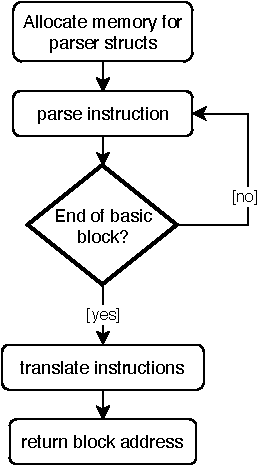
\includegraphics[width=0.7\textwidth]{diagrams/blocktranslate}
	\end{column}
\end{columns}
\end{frame}

\begin{frame}[fragile]
	\frametitle{Block Translator}
	\framesubtitle{Ausführung}
	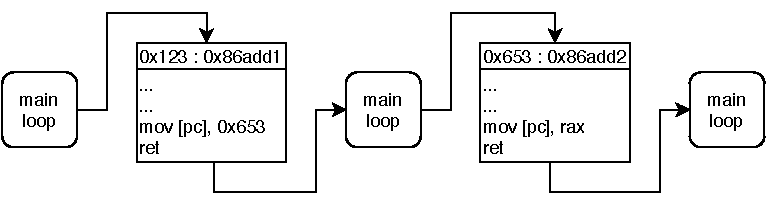
\includegraphics[width=0.99\textwidth]{diagrams/unchained}\\
	\vspace{1cm}
	\textbf{$\Rightarrow$} Overhead durch Rücksprung zu main
\end{frame}

\begin{frame}[fragile]
	\frametitle{Block Translator}
	\framesubtitle{Optimierungen}
	\begin{columns}
		\begin{column}{0.5\textwidth}
		\textbf{Ziel:} weniger Overhead durch main loop und Cache Lookup \\
		\onslide<2->
		\vspace{0.5cm}
		\textbf{Ansatz 1:} Jumps beim Parsen folgen: \\		Zieladresse auswerten und weiter parsen \\
		\onslide<3->
		\vspace{0.5cm}
		\textbf{Vorher:} \\
		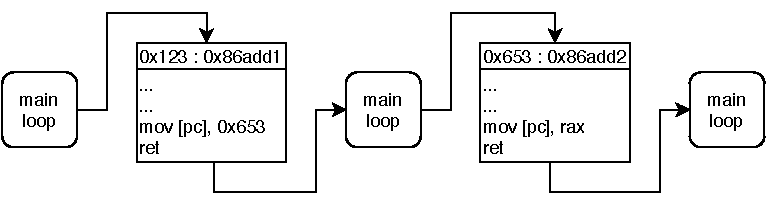
\includegraphics[width=0.99\textwidth]{diagrams/unchained}\\
		\onslide<5->
		\vspace{1cm}
		\textbf{Nachteil:} Mehrfachübersetzung von z.B. Funktionen \\
		\onslide<6->
		\textbf{$\Rightarrow$} nur für Jumps, nicht für Calls
		\end{column}
		\begin{column}{0.5\textwidth}
		\onslide<4->
		\textbf{Nachher:}\\
		\vspace{0.5cm}
		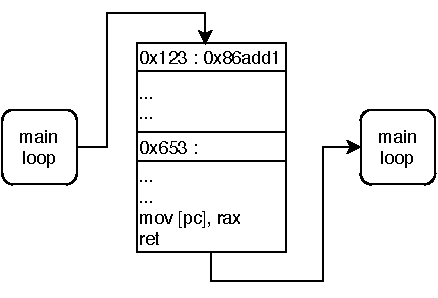
\includegraphics[width=0.78\textwidth]{diagrams/jal_follow}
		\end{column}
	\end{columns}
\end{frame}

\begin{frame}[fragile]
	\frametitle{Block Translator}
	\framesubtitle{Optimierungen}
	\textbf{Ziel:} weniger Overhead durch main loop und Cache Lookup \\
	\vspace{0.5cm}
	\textbf{Ansatz 2:} Basic Blocks verketten: \\ Direkt zum nächsten Block springen \\
	\onslide<2>
	\vspace{0.5cm}
	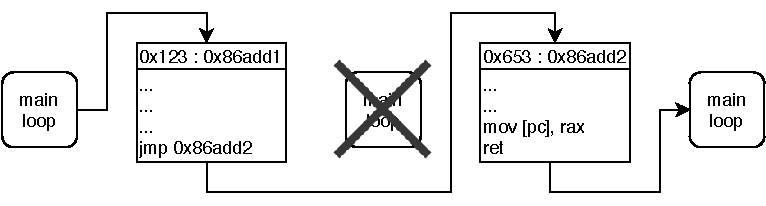
\includegraphics[width=0.7\textwidth]{diagrams/chained}
\end{frame}

\begin{frame}[fragile]
	\frametitle{Block Translator}
	\framesubtitle{Optimierungen}
	\textbf{Ziel:} weniger Overhead durch main loop und Cache Lookup \\
	\vspace{0.5cm}
	\textbf{Ansatz 2:} Basic Blocks verketten: \\ Direkt zum nächsten Block springen \\
	\vspace{0.5cm}
	\textbf{Voraussetzungen:}\\
	\begin{itemize}
		\item Statisches Sprungziel
		\item 2. Block bei Übersetzen von Block 1 bereits im Cache
	\end{itemize}
\end{frame}

\begin{frame}[fragile]
	\frametitle{Block Translator}
	\framesubtitle{Optimierungen}
	\textbf{Ziel:} weniger Overhead durch main loop und Cache Lookup \\
	\vspace{0.5cm}
	\textbf{Ansatz 2:} Basic Blocks verketten: \\ Direkt zum nächsten Block springen \\
	\vspace{0.5cm}
	\textbf{Was tun wenn 2. Block nicht im Cache?}\\
	\begin{itemize}
		\onslide<2->
		\item rekursives Übersetzen des Sprungziels beim Parsen
		\begin{itemize}
			\item[$\rightarrow$] Sprungziel ist beim Übersetzen im Cache
			\item[-] mögliche Rekursionsschleife $\rightarrow$ "translation started"-Flag im Cache benötigt
		\end{itemize}
		\onslide<3->
		\item RET anhängen $\rightarrow$ main loop
		\onslide<4->
		\item nachträgliches Verketten im main loop
		\begin{itemize}
			\item[-] zusätzlicher Pointer auf Ende des Blocks im Cache-Eintrag benötigt
		\end{itemize}
	\end{itemize}
\end{frame}


\subsection{Code Generator} % Flo
\begin{frame}[fragile]
	\frametitle{Dynamische Codegenerierung}
	\framesubtitle{Überblick}

	\textbf{Input:} geparste RISC-V-Instruktionen eines Basic Blocks\\
	\textbf{Output:} übersetzte x86-Instruktionen für diesen Block

	\pause
	\begin{columns}
		\begin{column}{0.5\textwidth}
			\vspace{0.25cm}
			\begin{itemize}
				\item Nutzen der Instruction-Structs des Parsers
				\item Instruktionsmapping RISC-V \refer x86
				\item einzelne Übersetzungsfunktionen für jede Instruktion
				
				\vspace{1cm}
				
				\item allokierte Speicherseite für die x86-Assembly
				\item Encoding der Instruktionen in den Speicherbereich
			\end{itemize}
		\end{column}
		
		\begin{column}{0.5\textwidth}
			\begin{lstlisting}
				typedef struct {
				    t_risc_addr addr;
				    t_risc_mnem mnem;
				    t_risc_optype optype;
				    t_risc_reg reg_src_1;
				    t_risc_reg reg_src_2;
				    t_risc_reg reg_dest;
				    t_risc_imm imm;
				} t_risc_instr;
			\end{lstlisting}
		\end{column}
	\end{columns}
\end{frame}

\begin{frame}[fragile]
	\frametitle{Dynamische Codegenerierung}
	\framesubtitle{Ansatz}
	
	Übersetzung aller Instruktionen im Basic Block in einen x86-Buffer,
	\begin{lstlisting}
		//aus translate_block(t_risc_addr), translate.cpp
		init_block();
		
		for (int i = 0; i < instructions_in_block; i++) {
			translate_risc_instr(block_cache[i], r_info);
    	}
    	
		return finalize_block();
	\end{lstlisting}
	
	anschließend
	\begin{itemize}
		\item Finalisieren des Blocks (\verb!ret! anhängen, etc.)
		\item Rückgabe des Blocks an den Cache (später).
	\end{itemize}
\end{frame}

\begin{frame}[fragile]
	\frametitle{Dynamische Codegenerierung}
	\framesubtitle{Metadaten}
	
	Register-Mapping als Parameter für die Übersetzerfunktionen, basierend auf Zuteilung des Block Loaders:
	\begin{lstlisting}
		/**
		 * Register information for the translator functions.
		 */
		struct register_info {
			FeReg *map;
			bool *mapped;
			uint64_t base;
		};
	\end{lstlisting}
	
	\begin{itemize}
		\item Synchronisierung der zugewiesenen Register mit register file
		\item Lesen/Schreiben an Basic-Block-Grenzen
		\item Unterschiedliche Instruktionsübersetzungen je nach Mapping
	\end{itemize}
\end{frame}

\begin{frame}[fragile]
	\frametitle{Dynamische Codegenerierung}
	\framesubtitle{Dispatch}
	
	Verteilung der Übersetzung auf einzelne Funktionen für jede Instruktion:
	
	\begin{lstlisting}
		//aus translate.cpp
		void translate_risc_instr(const t_risc_instr &instr, const register_info &r_info) {
			switch (instr.mnem) {
				//...
				case OR:
					translate_OR(instr, r_info);
					break;
				case AND:
					translate_AND(instr, r_info);
					break;
				case SLLIW:
					translate_SLLIW(instr, r_info);
					break;
				//...
		}
	\end{lstlisting}
\end{frame}

\begin{frame}[fragile]
	\frametitle{Dynamische Codegenerierung}
	\framesubtitle{Übersetzerfunktionen (1)}
	
	Realisierung der RISC-V-Instruktionen mit x86-64-Assembly.
	
	\pause
	\vspace{0.3cm}
	Einfache Instruktionen, z.B. \verb!ADD!:
	\begin{lstlisting}
		//aus translate_arithmetic.cpp
		void translate_ADD(const t_risc_instr &instr, const register_info &r_info) {
			if (r_info.mapped[instr.reg_dest] && r_info.mapped[instr.reg_src_1] && r_info.mapped[instr.reg_src_2]) {
				//...
			} else {
				err |= fe_enc64(&current, FE_MOV64rm, FE_AX, FE_MEM_ADDR(r_info.base + 8 * instr.reg_src_1));
				err |= fe_enc64(&current, FE_ADD64rm, FE_AX, FE_MEM_ADDR(r_info.base + 8 * instr.reg_src_2));
				err |= fe_enc64(&current, FE_MOV64mr, FE_MEM_ADDR(r_info.base + 8 * instr.reg_dest), FE_AX);
			}
		}
	\end{lstlisting}
	
	\refer Load-Store-Architektur vs. Register-Memory-Architecture
\end{frame}

\begin{frame}[fragile]
	\frametitle{Dynamische Codegenerierung}
	\framesubtitle{Übersetzerfunktionen (2)}
	
	Realisierung der RISC-V-Instruktionen mit x86-64-Assembly.
	
	\vspace{0.3cm}
	Notwendigkeit von Fallunterscheidungen, z.B. \verb!REM!: (Semantik nach \footfullcite{riscv-spec}, S. 44f.)
	\pause
	\begin{verbatim}
		mov rax, [r_info.base + 8 * instr.reg_src_1]
		cmp qword ptr [r_info.base + 8 * instr.reg_src_2], 0
		jnz not_div_zero
		mov [r_info.base + 8 * instr.reg_dest], rax
		jz div_zero
		
		not_div_zero:
		xor rdx, rdx
		idiv qword ptr [r_info.base + 8 * instr.reg_src_2]
		mov [r_info.base + 8 * instr.reg_dest], rdx
		
		div_zero:
	\end{verbatim}
\end{frame}

\begin{frame}[fragile]
	\frametitle{Dynamische Codegenerierung}
	\framesubtitle{Übersetzerfunktionen (3)}
	
	Realisierung der RISC-V-Instruktionen mit x86-64-Assembly.
	
	\vspace{0.3cm}
	Emulierung der system calls für \verb!ECALL!:
	\pause
	\begin{lstlisting}
		void translate_ECALL(const t_risc_instr &instr, const register_info &r_info) {
			save_risc_registers(r_info);
			err |= fe_enc64(&current, FE_MOV64ri, FE_DI, instr.addr);
			err |= fe_enc64(&current, FE_MOV64ri, FE_SI, r_info.base);
			typedef void emulate(t_risc_addr addr, t_risc_reg_val *registerValues);
			emulate *em = &emulate_ecall;
			err |= fe_enc64(&current, FE_CALL, reinterpret_cast<uintptr_t>(em));
		}
	\end{lstlisting}
	
	\begin{itemize}
		\item Behandlung von system calls zur Laufzeit
		\item Übersetzung, Adaptieren bzw. Emulieren der benötigten Funktionalität
	\end{itemize}
\end{frame}

\subsection{Code Cache} % Flo
\begin{frame}
	\frametitle{Code Cache}
	\framesubtitle{Überblick}
	
	\textbf{Ziel:} Caching bereits übersetzter Basic Blocks für nochmalige Ausführung (teure Übersetzung nur einfach)
	
	\pause
	\begin{figure}
		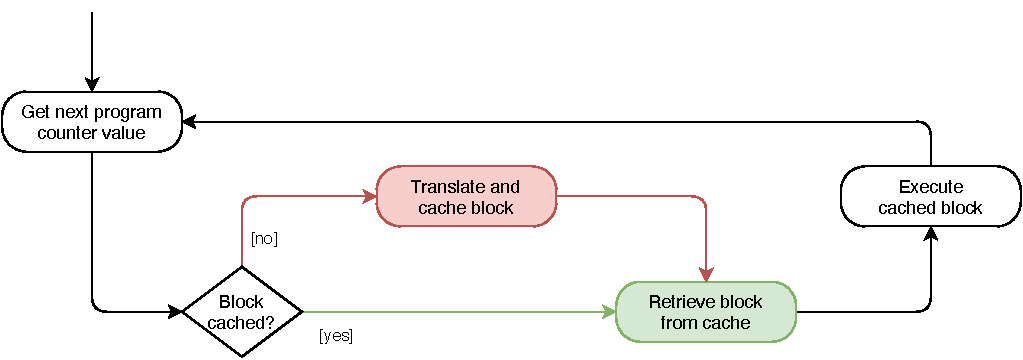
\includegraphics[width=0.95\textwidth]{diagrams/cache-flow}
	\end{figure}
\end{frame}

\begin{frame}[fragile]
	\frametitle{Code Cache}
	\framesubtitle{Ansatz}
	
	\textbf{Ziel:} Caching bereits übersetzter Basic Blocks für nochmalige Ausführung (teure Übersetzung nur einfach)
	
	\textbf{Idee:} Hashtable für schnellen Lookup der Blöcke, Startadresse des RISC-V-Blocks als Key
	
	\vspace{0.5cm}
	\pause
	Einträge speichern RISC-V-Blockstartadresse sowie die Adresse des übersetzten Blocks:
	\begin{lstlisting}
		typedef struct {
			t_risc_addr risc_addr;
			t_cache_loc cache_loc;
		} t_cache_entry;
	\end{lstlisting}
	
	\pause
	Lookup als Open Hashing mit linearem Sondieren, via
	\begin{lstlisting}
		inline size_t hash(t_risc_addr risc_addr) {
			return (risc_addr & 0x00003FFCu) >> 2u;
		}
	\end{lstlisting}
\end{frame}

\begin{frame}[fragile]
	\frametitle{Code Cache}
	\framesubtitle{Einsatz im System}
	
	Zugriff auf den Cache von außen via
	\begin{lstlisting}
		t_cache_loc lookup_cache_entry(t_risc_addr risc_addr);
		void set_cache_entry(t_risc_addr risc_addr, t_cache_loc cache_loc);
	\end{lstlisting}
	
	wobei \verb!UNSEEN_CODE! von \verb!lookup_cache_entry(...)! einen nicht im Cache enthaltenen Block anzeigt.
	
	\refer Dynamische Reallokation der Größe bei Kapazitätsgrenzen
	
	\vspace{0.5cm}
	\pause
	Ausführung bereits übersetzter Blöcke via
	\begin{lstlisting}
		typedef void (*blk)(void);
		((blk) loc)();
	\end{lstlisting}
\end{frame}


\section{Demo}
\begin{frame}[fragile, c]
	\frametitle{Demo}

	\begin{center}
		\Huge \texttt{./translator -f <binary>}
	\end{center}
\end{frame}
\end{document}
